\documentclass[12pt, a4paper]{article}
\usepackage[a4paper,
left=15mm,
right=15mm,
top=15mm,
bottom = 5mm]{geometry}
\usepackage{amsmath}
\usepackage{graphicx}
\usepackage{algorithm}
\usepackage{algorithmic}
\usepackage{multicol}
\usepackage{amsthm}
\usepackage{bm}
\usepackage{fancyhdr}
\usepackage{amssymb}
\usepackage{pifont}
\usepackage{array}

\newcommand{\cmark}{\ding{51}}%
\newcommand{\xmark}{\ding{55}}%

\newcolumntype{P}[1]{>{\centering\arraybackslash}p{#1}}  %per centrare le colonne nelle tabelle
\newcolumntype{M}[1]{>{\centering\arraybackslash}m{#1}} %per centrare le righe nelle tabelle
\renewcommand{\arraystretch}{1.2} 

\newcommand\tab[1][1cm]{\hspace*{#1}}
\renewcommand{\labelitemii}{$\star$}

\begin{document}


\begin{titlepage}
	\begin{center}
		\vspace*{1cm}

		\Huge{Tesina\\Human Computer Interaction}
		\vspace{1.5cm}
		\Huge
		\textbf{\\CiakTime}
		\vspace{1.5cm}

		\Large
		Authors:\\
		\textbf{Mauro Ficorella 1941639}\\
		\textbf{Martina Turbessi 1944497}\\
		\textbf{Valentina Sisti 1952657}\\
		\vspace{0.5cm}

		\vfill

		
\includegraphics[width=0.4\textwidth]{Images/Logo.jpg}

		\vfill

		\vspace{0.8cm}

		\Large
		Sapienza\\
		July 2021
	\end{center}
\end{titlepage}

\tableofcontents{}

% INTRODUZIONE --------------------------------------------------------------------

\newpage

\section{Introduction}

The idea behind CiakTime comes from the fact that nowadays there are a lot of movies out
both in theatres and in streaming platforms, so that cinema lovers can satisfy their
needs to stay updated with the latest movies and keep track of them.
Also they may want to know on which streaming platforms they can found the movies.
Finally they could have the necessity to interact with other cinema lovers about their
favourite movies or share their opinion about the movie with the community through reviews.
\\\\
For these reasons, our app offers a lot of functionalities.
The user has the possibility to keep track of already watched movies, movies to watch and favourite movies;
moreover he can search for movies by title, also filtering results, search for actors and movie directors,
look for upcoming movies and popular movies and actors.
Regarding the movies, he can read information about plot, cast, year of release, duration, genre,
movie director and streaming platform on which the movie is available; in addition, he can
review and rate movies, comment and like reviews made by other users.
Finally, regarding movie directors and actors, the user can read their biography and take a look to their
filmography.
\\\\
In order to involve as much users as possible, we decided to make our app available for both iOS and Android devices.





% Requirement analysis -------------------------------------------------------------------------

\newpage

\section{Requirement analysis}

\subsection{Competitor analysis}
We found two main competitors for our application: IMDb and Cinemaniac.
\paragraph{IMDb}\mbox{}\\\\

\includegraphics[width=0.4\textwidth]{Images/IMDb.png}\\
IMDb is the world's most popular and authoritative source for movie, TV, and celebrity information. This app has a
huge fanbase and a limitless cinema database.
On this app the user can watch trailers, get showtimes, and buy tickets for upcoming films. He can rate and review shows he has seen
and track what he wants to watch using his Watchlist, and he can also get suggestions regarding movies based on it.\\
However, we have identified few weaknesses, such as the impossibility to exchange opinions between users, to keep track
of already watched movies and to save favourite movies in a list; it is also not very intuitive to retrieve movies specific
information due to the high number of functionality offered by the application.

\paragraph{Cinemaniac}\mbox{}\\\\

\includegraphics[width=0.4\textwidth]{Images/Cinemaniac.png}\\
Cinemaniac is an app on which the user can search for a movie and add it to the “Movies to watch”, “Watched movies” or favourite list.
He can see all the relevant details for any movie and he can leave his own personal grade.
The user can find suggestions on the most popular and top rated movies.
Moreover, he can find a specific list relative to currently projected movies and upcoming titles.\\
Also here we have identified some weaknesses, like the fact that the interface is not so user friendly, there is no user interaction,
there are no information about streaming platforms; moreover the search about movies is not so intuitive and there are
in-app purchases required to remove advertisements and unlock some functionalities.\\\\
In the following table we summarize the comparison between our app and the competitors:

\begin{center}
	\begin{tabular}{ |p{5cm}|P{3cm}|P{3cm}|P{3cm}|  }
		\cline{2-4}
		\multicolumn{1}{c|}{}
		                               & \textbf{CiakTime} & \textbf{IMDb} & \textbf{Cinemaniac} \\
		\hline
		\textbf{User profile}          & \checkmark        & \checkmark    & \xmark              \\
		\hline
		\textbf{Search}                & \checkmark        & \checkmark    & \checkmark          \\
		\hline
		\textbf{Movie info}            & \checkmark        & \checkmark    & \checkmark          \\
		\hline
		\textbf{Streaming platform}    & \checkmark        & \checkmark    & \xmark              \\
		\hline
		\textbf{Upcoming movies}       & \checkmark        & \checkmark    & \checkmark          \\
		\hline
		\textbf{Watch history}         & \checkmark        & \xmark        & \checkmark          \\
		\hline
		\textbf{Watch list}            & \checkmark        & \checkmark    & \checkmark          \\
		\hline
		\textbf{Favourite movies}      & \checkmark        & \xmark        & \checkmark          \\
		\hline
		\textbf{Review movies}         & \checkmark        & \checkmark    & \checkmark          \\
		\hline
		\textbf{Rate movies}           & \checkmark        & \checkmark    & \checkmark          \\
		\hline
		\textbf{Comment other reviews} & \checkmark        & \xmark        & \xmark              \\
		\hline
		\textbf{Like other reviews}    & \checkmark        & \checkmark    & \xmark              \\
		\hline
		\textbf{No ads}                & \checkmark        & \checkmark    & \xmark              \\
		\hline
	\end{tabular}
\end{center}


\subsection{User analysis}
In this section we want to analyze the possible users for our application.
In particular we describe the User Profile, which is a detailed description of our users'
attributes, the Personas, which are fictional individuals created to describe the typical user
based on the user profile and the Scenarios, which are stories that describe how a particular
persona completes a task or behaves in a given situation.

\subsubsection{User Profile}

\begin{center}
	\begin{tabular}{ |p{3cm}|P{7cm}|  }
		\hline
		\textbf{Age}        & 18-50 years                 \\
		\hline
		\textbf{Gender}     & male/female                 \\
		\hline
		\textbf{Profession} & Any                         \\
		\hline
		\textbf{Education}  & Any                         \\
		\hline
		\textbf{Location}   & Any                         \\
		\hline
		\textbf{Tecnology}  & Basic smartphone experience \\
		\hline
		\textbf{Passions}   & Cinema, movies              \\
		\hline
	\end{tabular}
\end{center}

\subsubsection{Persona 1 - Vittoria}

\begin{minipage}{0.25\textwidth}
	
\includegraphics[width=1\textwidth]{images/vittoria.png}
\end{minipage}
\hspace{0.02\linewidth}
\begin{minipage}{0.7\textwidth}
	\textbf{Age:} 25 years-old \\
	\textbf{Gender:} Female\\
	\textbf{Profession:} Student\\
	\textbf{Education:} University student\\
	\textbf{Location:} Rome, Italy\\
	\textbf{Tecnology:} Mid level\\
	\textbf{Passions:} Watching movies and tv-series on streaming platforms \\
\end{minipage}

\paragraph{Persona}\mbox{}\\
Vittoria is 25 years-old and comes from Rome. She is a university student and in the free
time her main hobby is watching movies and tv-series on her favourite streaming platforms.
During her study breaks she likes to keep in touch with her friends on various social apps.

\paragraph{Scenario}\mbox{}\\
Vittoria has just terminated an intense study session and now she only wants to
relax watching a movie. She decides to call her best friend to spend the evening together.
Once she arrives, in order to choose which movie to watch, they both open the app to
compare their watchlists. After a while they realize that both have “La La Land“ in their
watchlists and so decide to watch it together.
At the end of the evening they both check it as “watched“ in their app.

\subsubsection{Persona 2 - Emanuele}

\begin{minipage}{0.25\textwidth}
	
\includegraphics[width=1\textwidth]{images/emanuele.png}
\end{minipage}
\hspace{0.02\linewidth}
\begin{minipage}{0.6\textwidth}
	\textbf{Age:} 33 years-old\\
	\textbf{Gender:} Male\\
	\textbf{Profession:} Programmer\\
	\textbf{Education:} Degree\\
	\textbf{Location:} Torino, Italy\\
	\textbf{Tecnology:} High level\\
	\textbf{Passions:} Action movies, technology\\
\end{minipage}

\paragraph{Persona}\mbox{}\\
Emanuele is 33 years-old and comes from Torino. He is a programmer and he likes
very much going to the cinema with his girlfriend.
As a programmer, he is addicted of technology in general, and more specific of mobile
devices; moreover he is a very organized guy, and so he likes to keep under control
everything he does in his life using mobile apps.

\paragraph{Scenario}\mbox{}\\
It is an afternoon autumn day. Emanuele and his girlfriend would have liked to go
out for a walk, but since it’s raining, they don’t know what to do. So, Emanuele opens
the app in search of new movies available in cinemas. In this list he founds that is just
available a new action movie with his favourite actor Vin Diesel; since also his
girlfriend likes action movies, they decide to go to the cinema to watch it and spend
a good afternoon together.



\subsection{Questionnaire analysis}

Questionnaires are a useful method to investigate user needs, expectations, perspectives, priorities and preferences.
They are useful in user requirement but also in evaluation phase to investigate user satisfaction, user attitudes and opinions, relevance of collections and services to user needs, trends.
We designed the questionnaire in such a way that each question was clearly written, in order to not lead the user to a specific answer and to
always make them feel confortable while answering.
Below we present the questionnaire results used to better understand the target of potential users in order to have a better refinement of
some aspects of our application.
More precisely, we reached 151 people, and so we had a good number of answers, statistically speaking.

\paragraph{What's your age?}\mbox{}\\\\
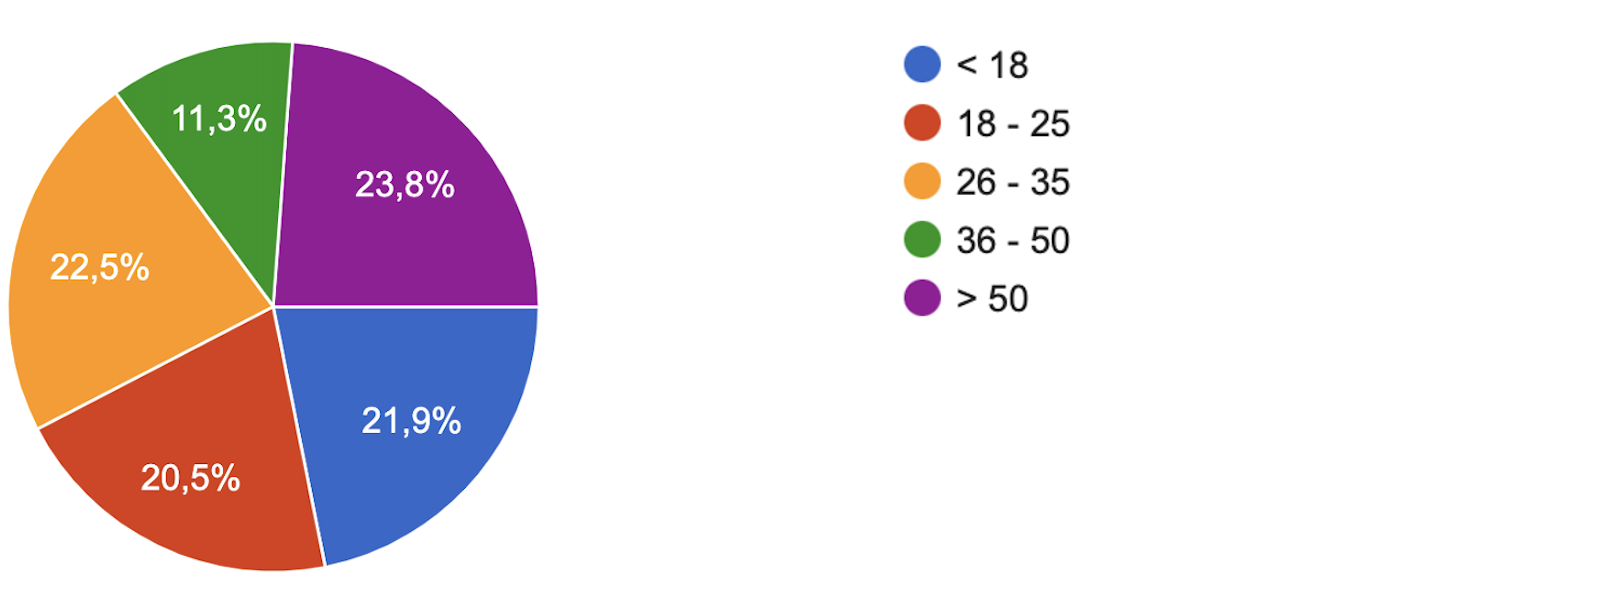
\includegraphics[width=0.7\textwidth]{Images/age.png}

\paragraph{What's your gender?}\mbox{}\\\\
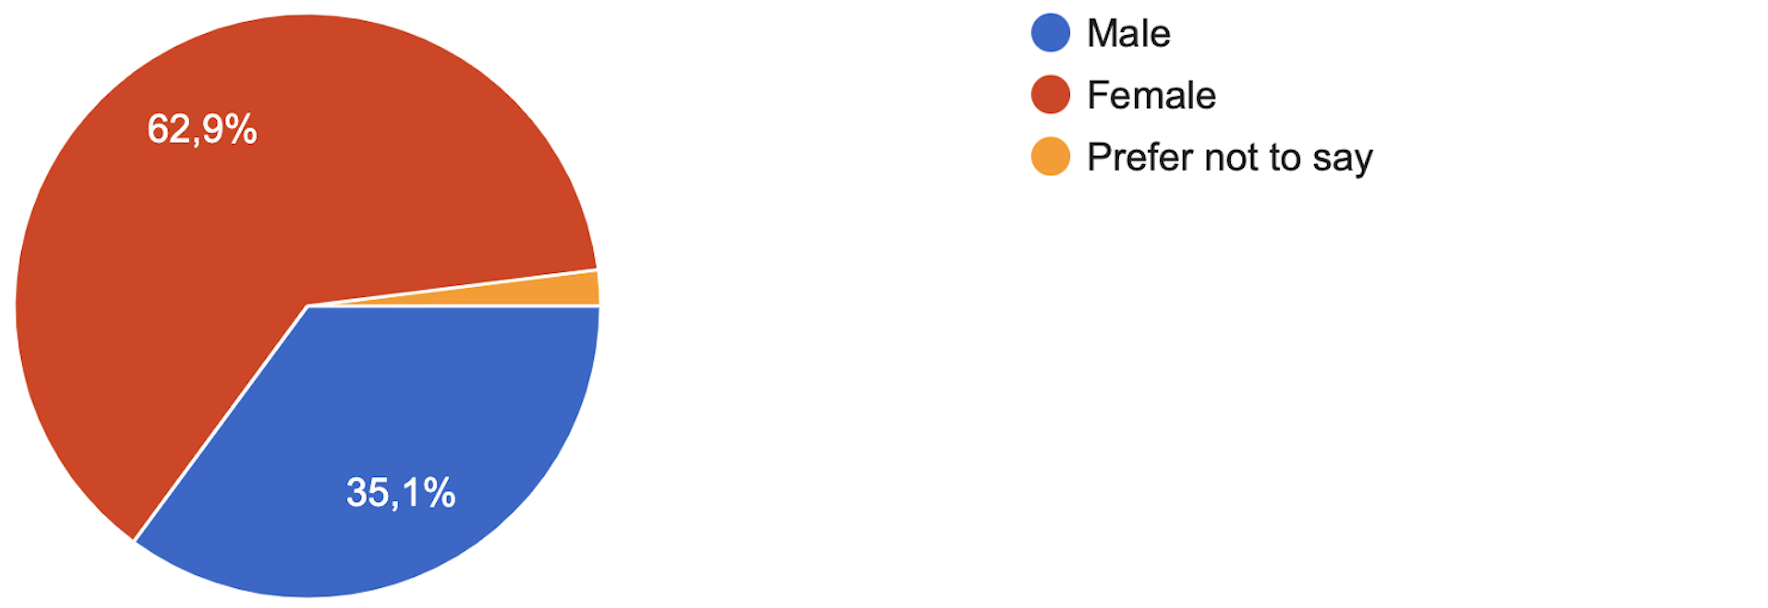
\includegraphics[width=0.7\textwidth]{Images/gender.png}

\paragraph{What's your educational level?}\mbox{}\\\\
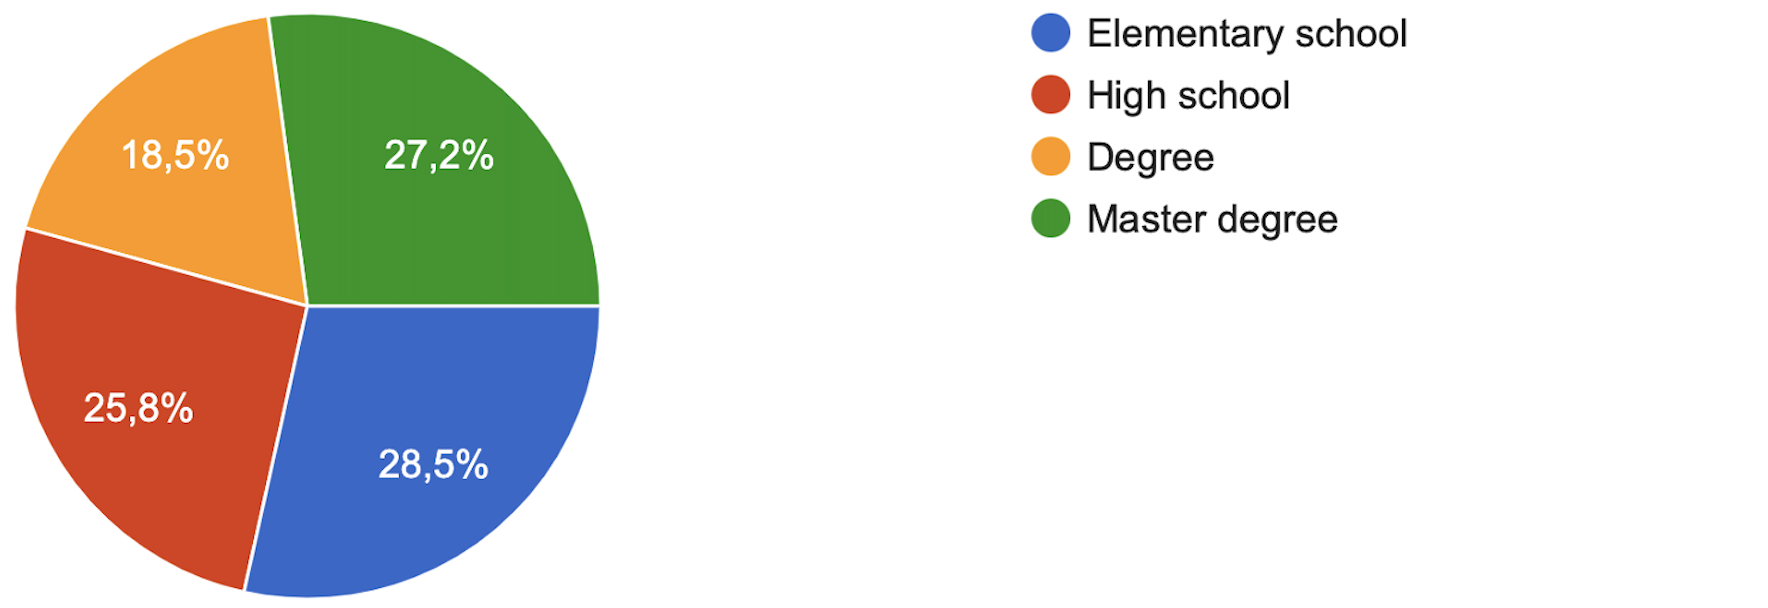
\includegraphics[width=0.7\textwidth]{Images/education.png}\\\\\\\\\\\\\\


\paragraph{How frequently do you use your smartphone on average?}\mbox{}\\\\
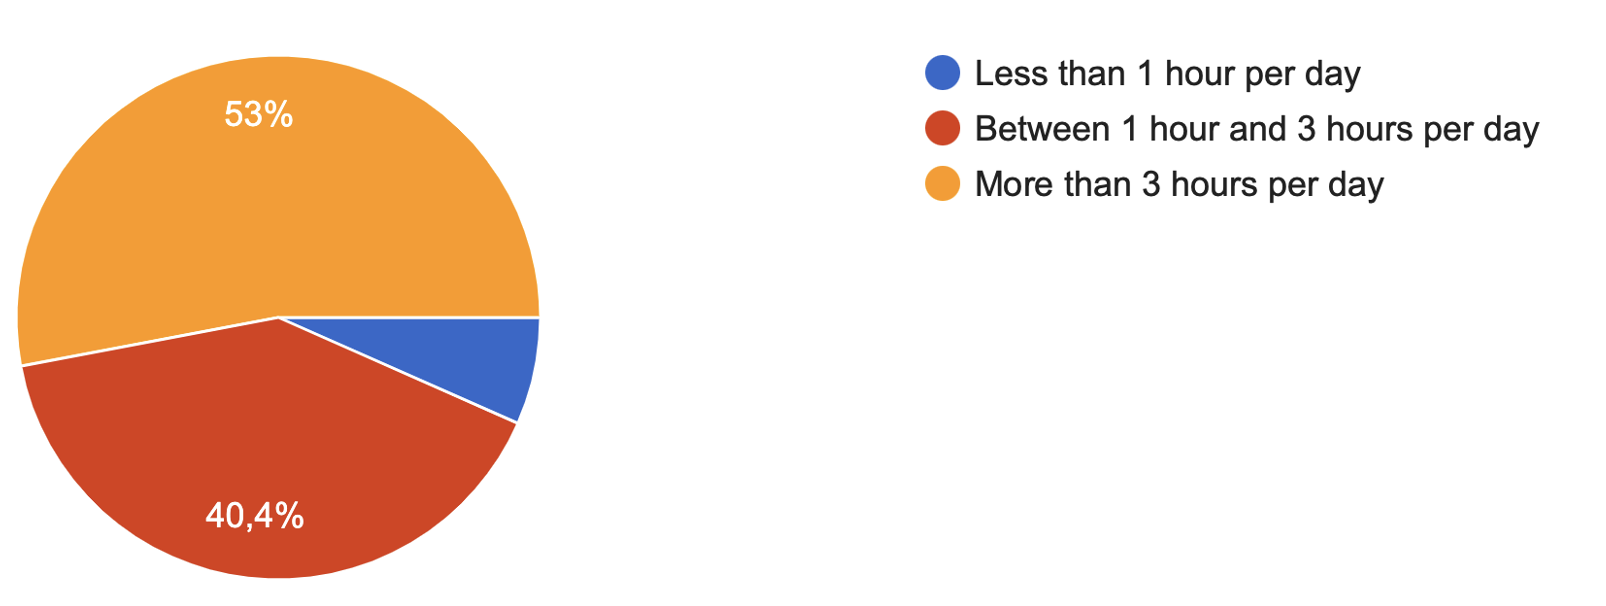
\includegraphics[width=0.7\textwidth]{Images/timeAtPhone.png}

\paragraph{How many times do you go to the cinema on average? (Before pandemic)}\mbox{}\\\\
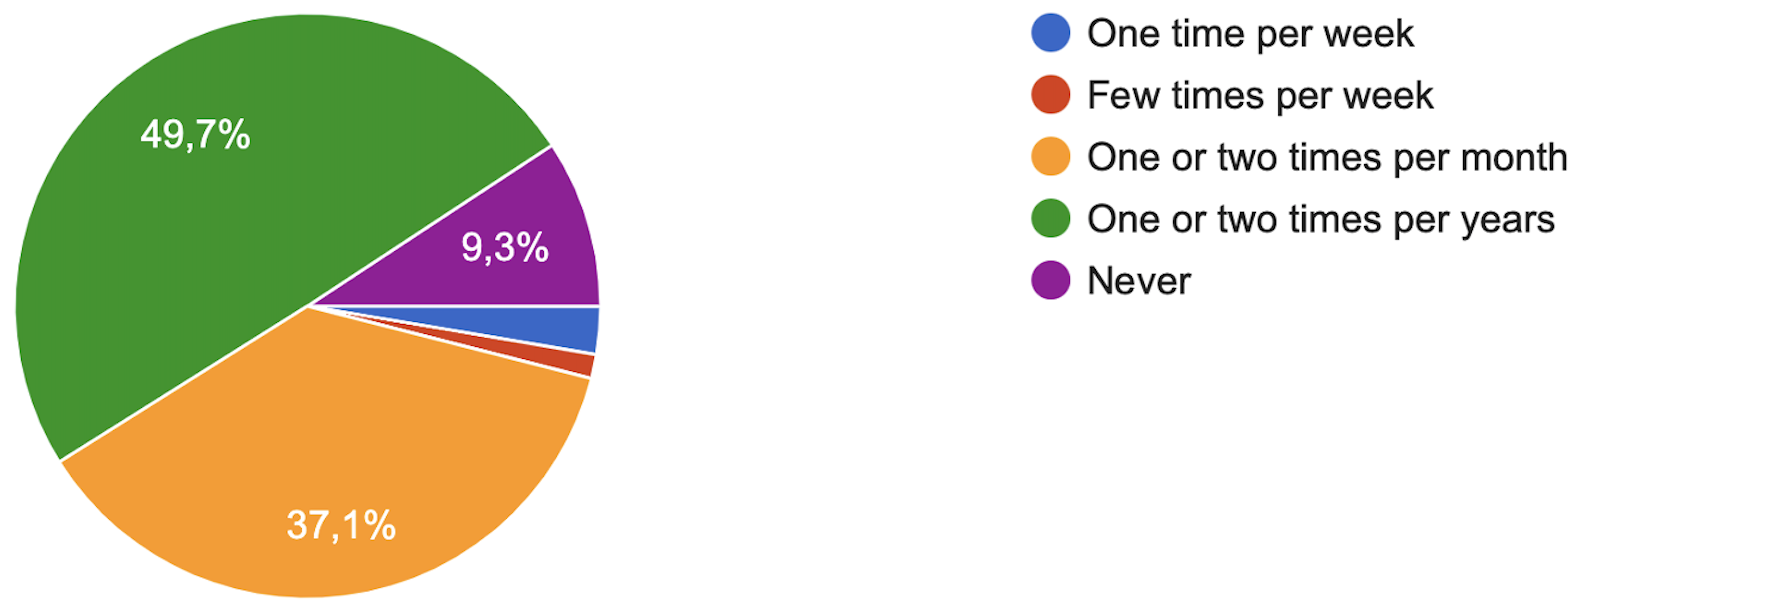
\includegraphics[width=0.7\textwidth]{Images/timeAtCinema.png}

\paragraph{How many times do you watch movies on streaming platforms/tv on average?}\mbox{}\\\\
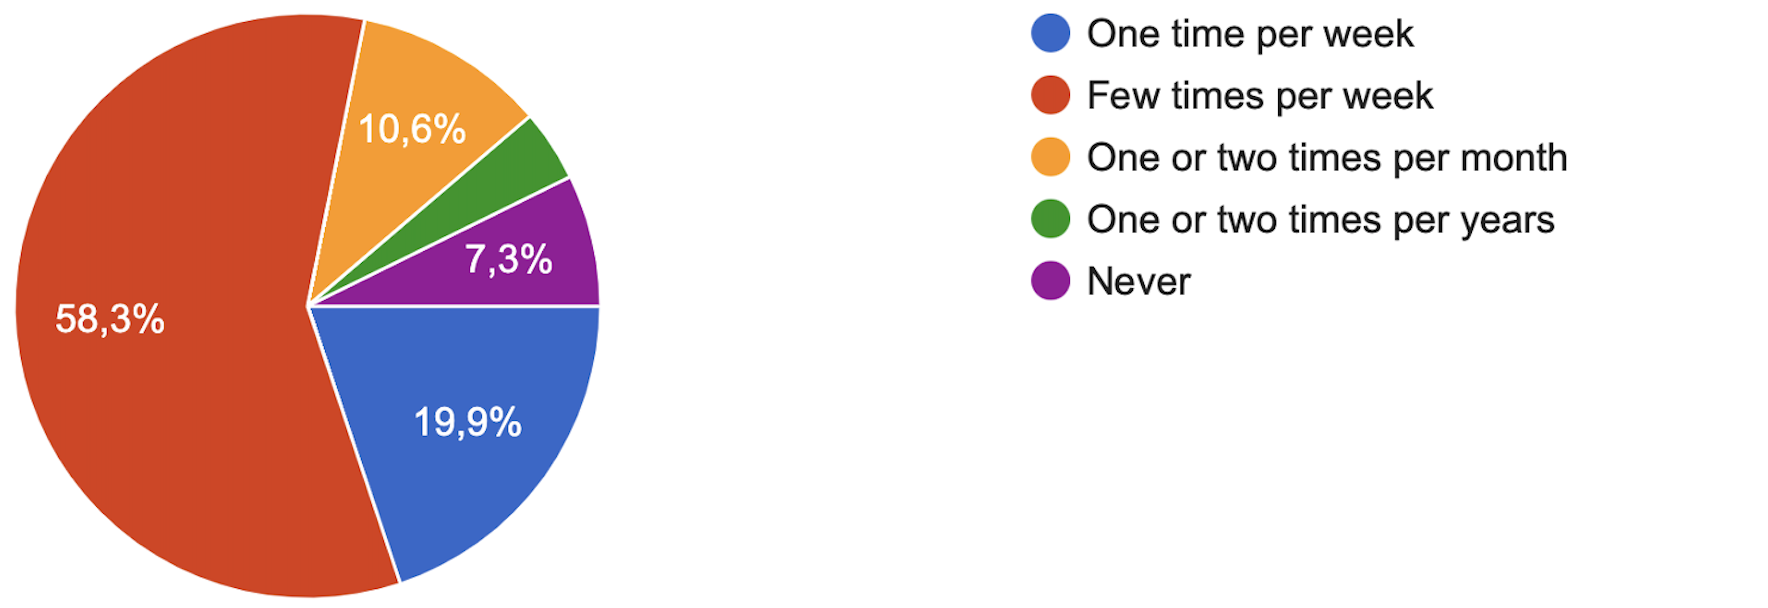
\includegraphics[width=0.7\textwidth]{Images/timeStreaming.png}

\paragraph{Which streaming platforms do you know?}\mbox{}\\\\
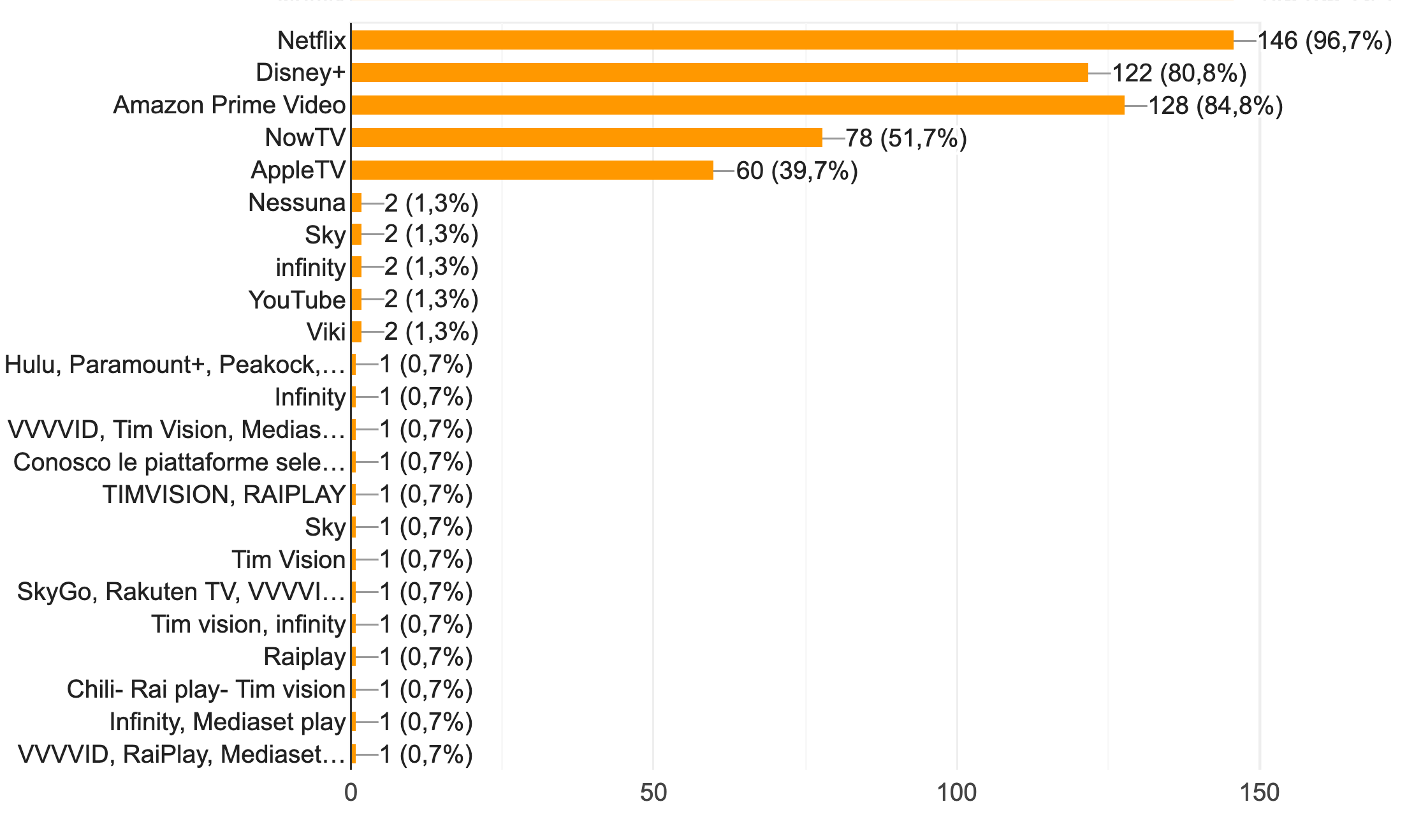
\includegraphics[width=0.7\textwidth]{Images/streamingPlatform.png}\\

\paragraph{Which streaming platforms do you use?}\mbox{}\\\\
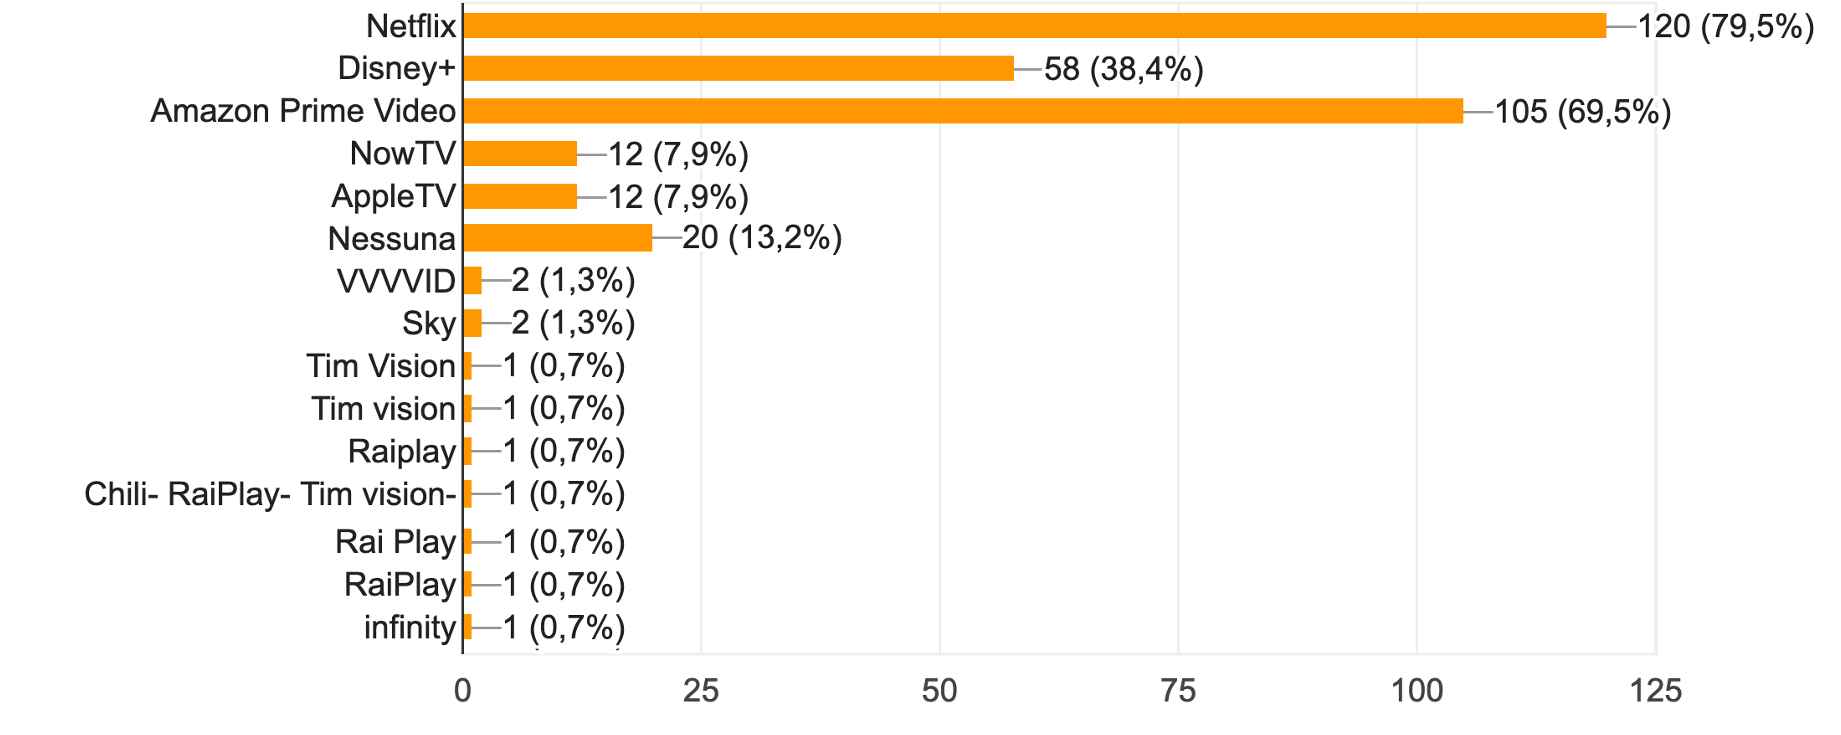
\includegraphics[width=0.7\textwidth]{Images/streamingPlatformUsed.png}

\paragraph{Do you use any movies related app?}\mbox{}\\\\
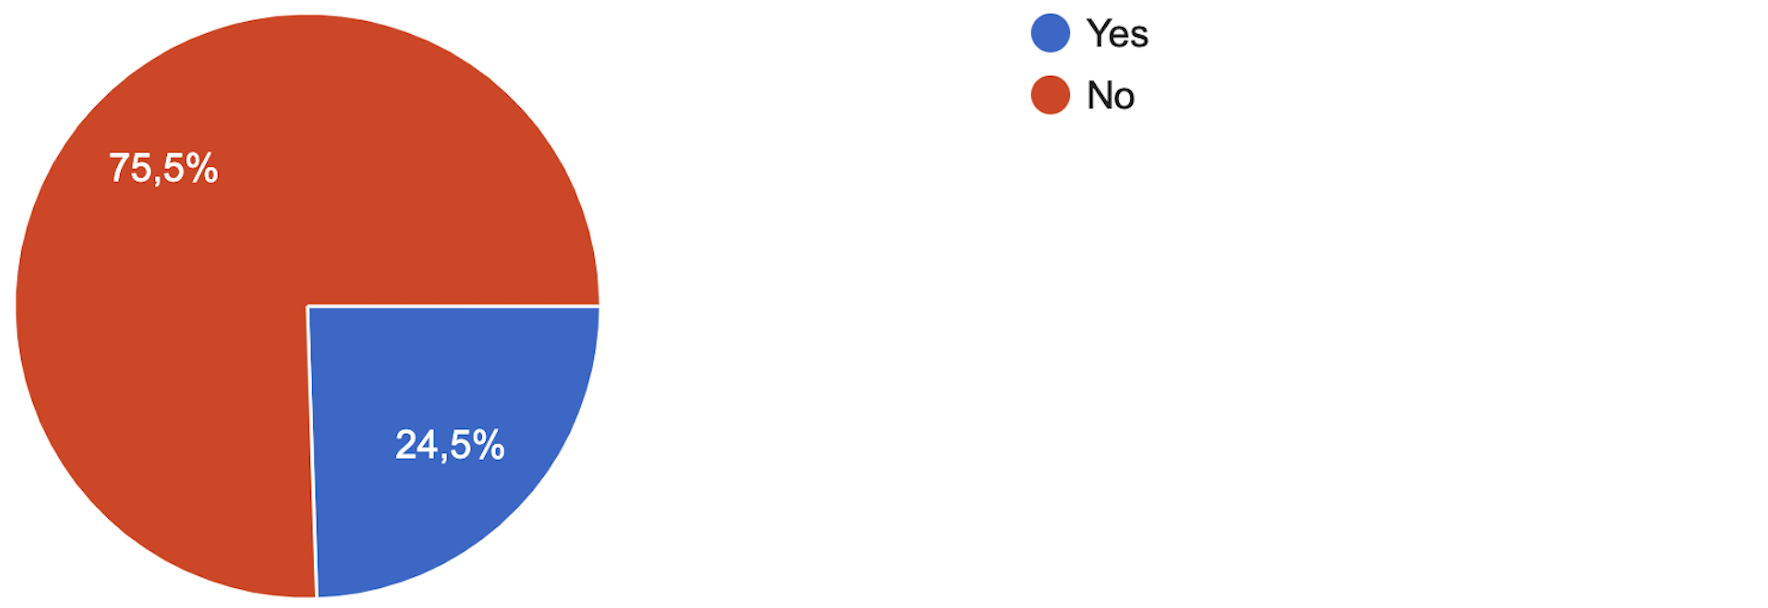
\includegraphics[width=0.7\textwidth]{Images/app.png}

\paragraph{If you use any movies related app, which one?}\mbox{}\\\\
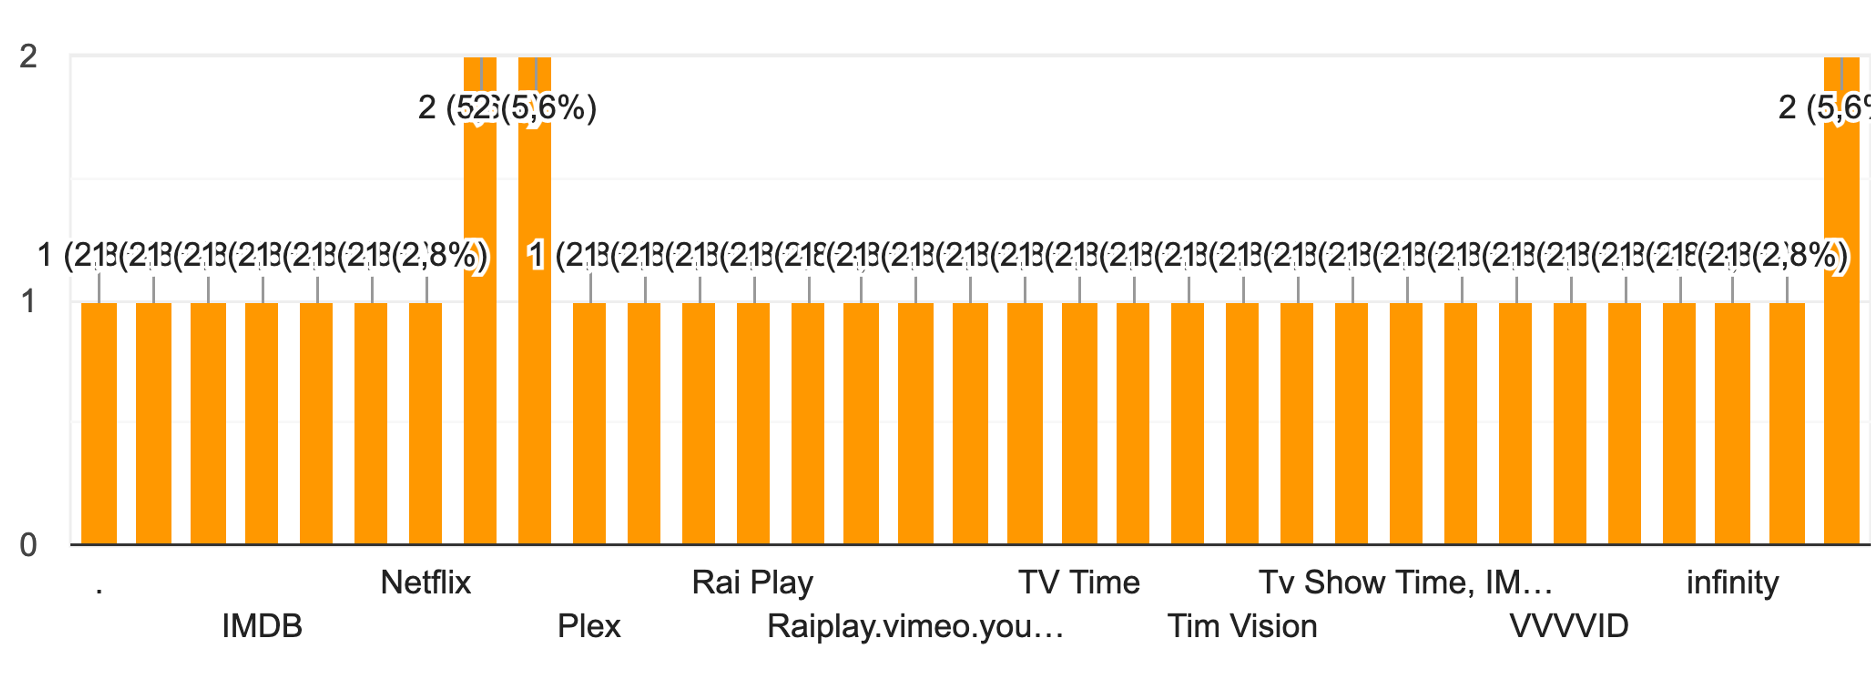
\includegraphics[width=0.7\textwidth]{images/appUsed.png}

\paragraph{If you don't use any movies related app, how much would you be interest in using one?}\mbox{}\\\\
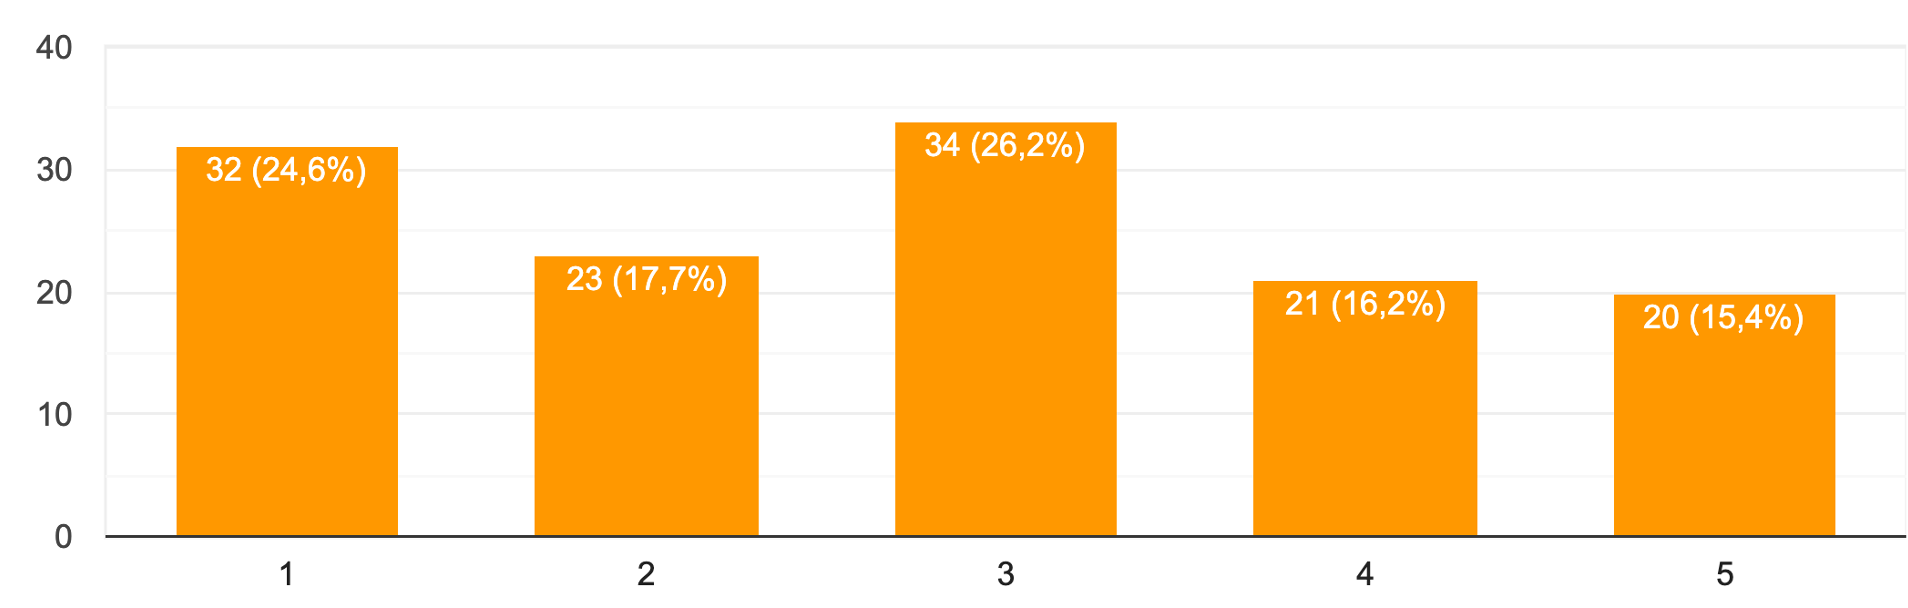
\includegraphics[width=0.7\textwidth]{images/interesting.png}\\\\\\\\\\

\paragraph{How much do you think the following features are important in such an app?}\mbox{}\\\\
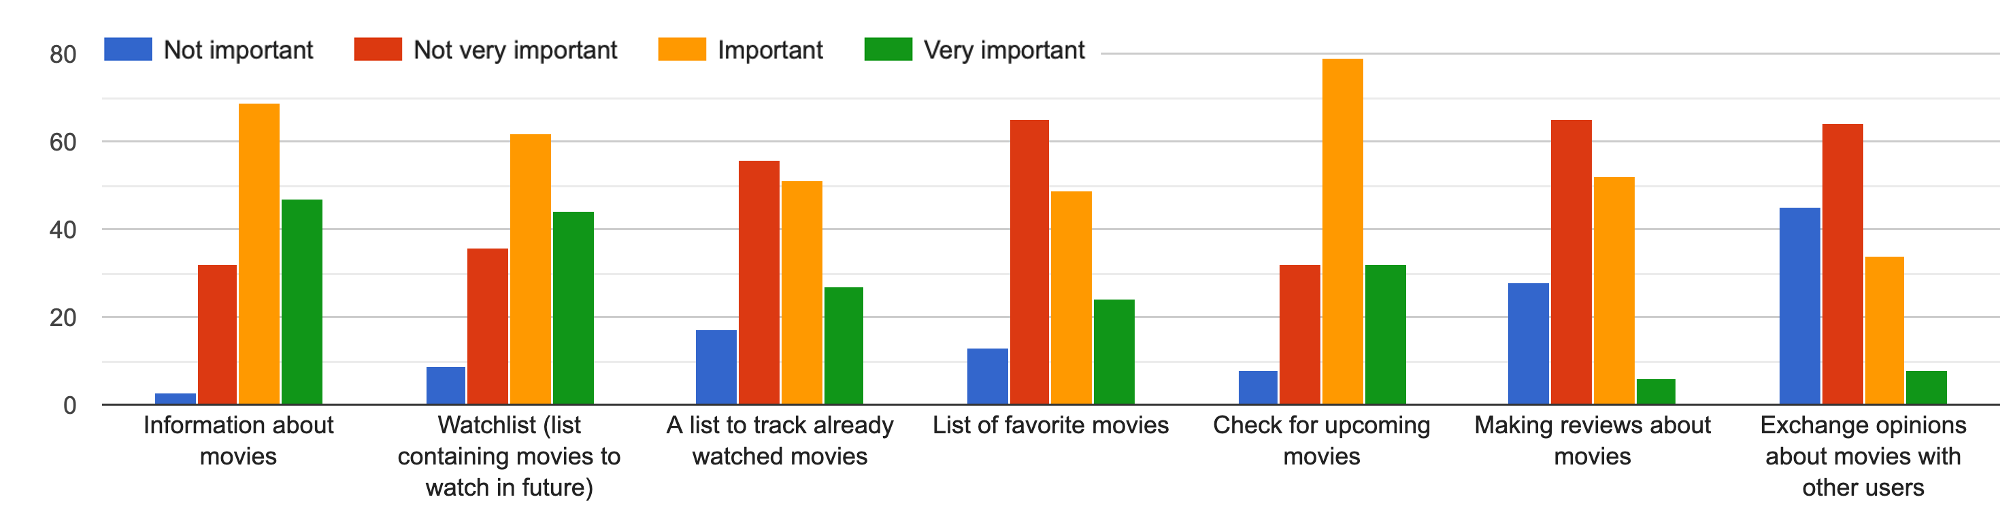
\includegraphics[width=1\textwidth]{Images/features.png}

\subsubsection{Conclusions}
After having analyzed the results obtained from the questionnaires, we have formalized the following conclusions:
\begin{itemize}
	\setlength\itemsep{0.01em}
	\item Regarding ages, we noticed that there is no predominant range, but they are more or less equally distributed between 18 and 50, and the majority of them are women.
	\item The majority of them uses smartphone more than 3 hours per day.
	\item Since we noticed that the majority of people rarely goes to cinema and conversely watches very often movies on streaming platform, we decided to focus our app on this feature.
	\item Moreover, given the fact that a very high number of people does not use a movie related app and that the majority of them would be interested in doing this, we thought that the idea of such an app would be very appreciated.
	\item Finally, from the last question, emerge the most wanted features such as have informations about movies, have the possibility to add movies to lists and have informations about upcoming movies, and so we decided to focused on them.
\end{itemize}



% CAPITOLO 2 -------------------------------------------------------------------------

\newpage

\section{Task analysis: HTA and STN}

% CAPITOLO 3 -------------------------------------------------------------------------

\newpage

\section*{NOME}

% CAPITOLO 4 -------------------------------------------------------------------------

\newpage

\section*{NOME}

% CAPITOLO 5 -------------------------------------------------------------------------

\newpage

\section*{NOME}

% CAPITOLO 6 -------------------------------------------------------------------------

\newpage

\section*{NOME}

% CAPITOLO 7 -------------------------------------------------------------------------

\newpage

\section*{NOME}

% CAPITOLO 8 -------------------------------------------------------------------------

\newpage

\section*{NOME}

\end{document}

% COSE UTILI --------------------------------------------------------------------------

%\section*{NOME}
%\subsection*{1.1}
%\setlength{\intextsep}{0pt} --> elimina lo spazio
%\vspace{-3mm}
%\hspace*{0cm}

% Font -------------------------------------

%GRASSETTO: \textbf

% Simboli ---------------------------------

%$\leftarrow$

% Elenco puntato ----------------------

%\begin{itemize}
%\setlength\itemsep{0.01em}
%\item 1
%\item 2
%\end{itemize}

% Graffa grande -----------------------

%\[  
%    \left\{ 
%    \begin{array}{ll} 
%      \mbox{1}
%      \mbox{2}
%    \end{array}
%    \mbox{riga al lato}
%   \right. 
%\]

% Multicolonne --------------------------

% \begin{multicols}{2}
% \columnbreak
% \end{multicols}

% Algoritmi -------------------------------

%\renewcommand{\thealgorithm}{1.\arabic{algorithm}}
%\setcounter{algorithm}{0}
%\begin{algorithm}
%\footnotesize
%\caption{Nome}
%\textbf{Input:} \\
%\textbf{Output:} 

%\begin{algorithmic}[1]
%\STATE 
%\FOR{ = 0 \TO i = n} ---- \ENDFOR
%\IF{} ---- \ELSIF{} ---- \ENDIF
%\RETURN 
%\end{algorithmic}
%\end{algorithm}

% Minipage ------------------------------

%\begin{minipage}[t]{0.5\textwidth}

% queste 3 righe vanno attaccate
%\end{minipage}
%\hspace{0.02\linewidth}
%\begin{minipage}[t]{0.47\textwidth} 

%\begin{minipage}[t]{0.3\textwidth} 
%\end{minipage}

% Proof --------------------------------
%\begin{proof}[\textbf{per cambiare nome}]
%\end{proof}

